\chapter{Analyse et Conception}

\section{Analyse des Besoins}

\subsection{Besoins fonctionnels}

\subsubsection{Gestion des colis}

La fonctionnalité de gestion des colis constitue le cœur métier du système et nécessite une approche exhaustive pour répondre aux exigences opérationnelles de Barid Al Maghrib. Le système doit permettre la consultation en temps réel des informations détaillées de chaque colis, incluant le code d'envoi unique, les coordonnées complètes du destinataire, l'adresse de livraison, le statut de traitement, les montants CRBT (Cash on Delivery), et l'historique complet des mouvements.

L'interface de listing des colis doit offrir des capacités de filtrage avancé permettant aux utilisateurs de localiser rapidement les envois selon multiple critères : plage de dates de dépôt, statuts de livraison, destinations géographiques, montants, et informations destinataires. Cette fonctionnalité doit supporter des volumes importants de données tout en maintenant des temps de réponse acceptables pour l'usage quotidien.

La gestion des modifications de colis représente un besoin fonctionnel critique nécessitant un workflow d'approbation structuré. Les clients doivent pouvoir soumettre des demandes de modification pour les informations non critiques (adresse, téléphone destinataire, CRBT), tandis que les administrateurs disposent de capacités de validation, rejet, ou approbation avec traçabilité complète des actions effectuées.

\subsubsection{Suivi et traçabilité}

Le système de suivi doit offrir une visibilité complète sur le parcours de chaque colis depuis son dépôt jusqu'à sa livraison finale. Cette fonctionnalité requiert l'affichage chronologique des différents statuts (déposé, en transit, en cours de livraison, livré, retourné) avec horodatage précis et localisation géographique quand disponible.

L'implémentation doit supporter la recherche multicritère permettant aux utilisateurs de localiser un colis par son code d'envoi, le nom ou téléphone du destinataire, ou l'adresse de livraison. Cette recherche doit intégrer des capacités de recherche floue pour compenser les erreurs de saisie ou les variations orthographiques courantes.

La traçabilité des actions administratives constitue un besoin réglementaire nécessitant la conservation de l'historique complet des consultations, modifications, et actions effectuées sur chaque colis, avec identification de l'utilisateur et horodatage précis.

\subsubsection{Interface utilisateur}

L'interface utilisateur doit s'adapter aux différents profils d'utilisateurs en proposant des vues spécialisées selon les rôles et responsabilités. L'interface client privilégie la simplicité et l'accès direct aux informations essentielles : liste des colis, détails individuels, recherche rapide, et demandes de modification.

L'interface administrative nécessite des fonctionnalités étendues incluant la gestion globale des colis tous clients confondus, les outils de validation des modifications, l'accès aux statistiques globales, et les fonctionnalités de supervision système.

La responsivité et l'adaptabilité multi-device constituent des exigences essentielles compte tenu de l'usage mobile fréquent dans les contextes opérationnels de Barid Al Maghrib. L'interface doit conserver sa fonctionnalité complète sur tablettes et smartphones tout en optimisant l'ergonomie pour chaque format d'écran.

\subsection{Besoins non fonctionnels}

\subsubsection{Performance}

Les exigences de performance constituent un défi technique majeur compte tenu des volumes de données traités quotidiennement par Barid Al Maghrib. Le système doit maintenir des temps de réponse inférieurs à 2 secondes pour l'affichage des listes de colis, même avec des jeux de données dépassant 50 000 enregistrements par client.

Les opérations de recherche textuelle doivent s'exécuter en moins de 1 seconde pour garantir la fluidité des interactions utilisateur. Cette exigence nécessite l'implémentation d'indexation full-text optimisée et de stratégies de cache appropriées pour les requêtes fréquentes.

La génération des rapports statistiques, particulièrement consommatrice en ressources, doit s'achever en moins de 10 secondes pour les synthèses standard et moins de 30 secondes pour les analyses approfondies couvrant plusieurs mois d'historique.

\subsubsection{Sécurité}

La sécurisation du système doit répondre aux standards enterprise et aux exigences réglementaires applicables au secteur postal. L'authentification doit s'appuyer sur des protocoles modernes (OAuth 2.0, OpenID Connect) avec support de l'authentification multi-facteur pour les comptes administrateurs.

La gestion des autorisations doit implémenter une séparation stricte entre les données des différents clients, garantissant qu'aucun utilisateur ne puisse accéder aux informations d'un autre client. Cette isolation doit être vérifiée à tous les niveaux : interface utilisateur, API, et base de données.

Le chiffrement des communications via HTTPS/TLS est obligatoire pour toutes les interactions entre les composants du système. Les données sensibles stockées en base doivent bénéficier de mesures de protection appropriées conformément aux bonnes pratiques de sécurité.

\subsubsection{Disponibilité}

Le système doit assurer une disponibilité minimale de 99,5\% durant les heures ouvrées, avec des fenêtres de maintenance planifiées en dehors des heures de forte activité. Cette exigence nécessite l'implémentation de mécanismes de tolérance aux pannes et de récupération automatique.

La robustesse face aux pics de charge constitue une priorité, le système devant maintenir ses performances durant les périodes de forte activité commerciale (fêtes, promotions e-commerce) où les volumes peuvent tripler par rapport à l'activité normale.

Les temps de récupération après incident ne doivent pas excéder 4 heures pour les pannes majeures et 1 heure pour les incidents mineurs, nécessitant des procédures de sauvegarde et de restauration rigoureusement testées.

\subsubsection{Maintenabilité}

L'architecture du système doit favoriser la maintenabilité à long terme à travers une séparation claire des responsabilités et une documentation technique exhaustive. Le code doit respecter les standards de qualité industriels avec une couverture de tests unitaires minimale de 80\%.

La modularité de l'architecture doit permettre l'évolution indépendante des différents composants sans impact sur l'ensemble du système. Cette approche facilite les mises à jour technologiques et l'ajout de nouvelles fonctionnalités selon les besoins métier évolutifs.

La monitoring et l'observabilité du système en production doivent être intégrés dès la conception, incluant la surveillance des performances, la détection d'anomalies, et l'alerting automatique pour les situations nécessitant une intervention technique.
\newpage
\section{Conception de l'Architecture}

\subsection{Architecture globale}

L'architecture conçue pour le système optimisé s'articule autour d'une approche hybride innovante combinant les avantages des bases de données relationnelles et NoSQL. Cette architecture en couches privilégie la séparation des préoccupations et la scalabilité horizontale pour répondre aux exigences de performance et de croissance de Barid Al Maghrib.

\begin{figure}[H]
\centering
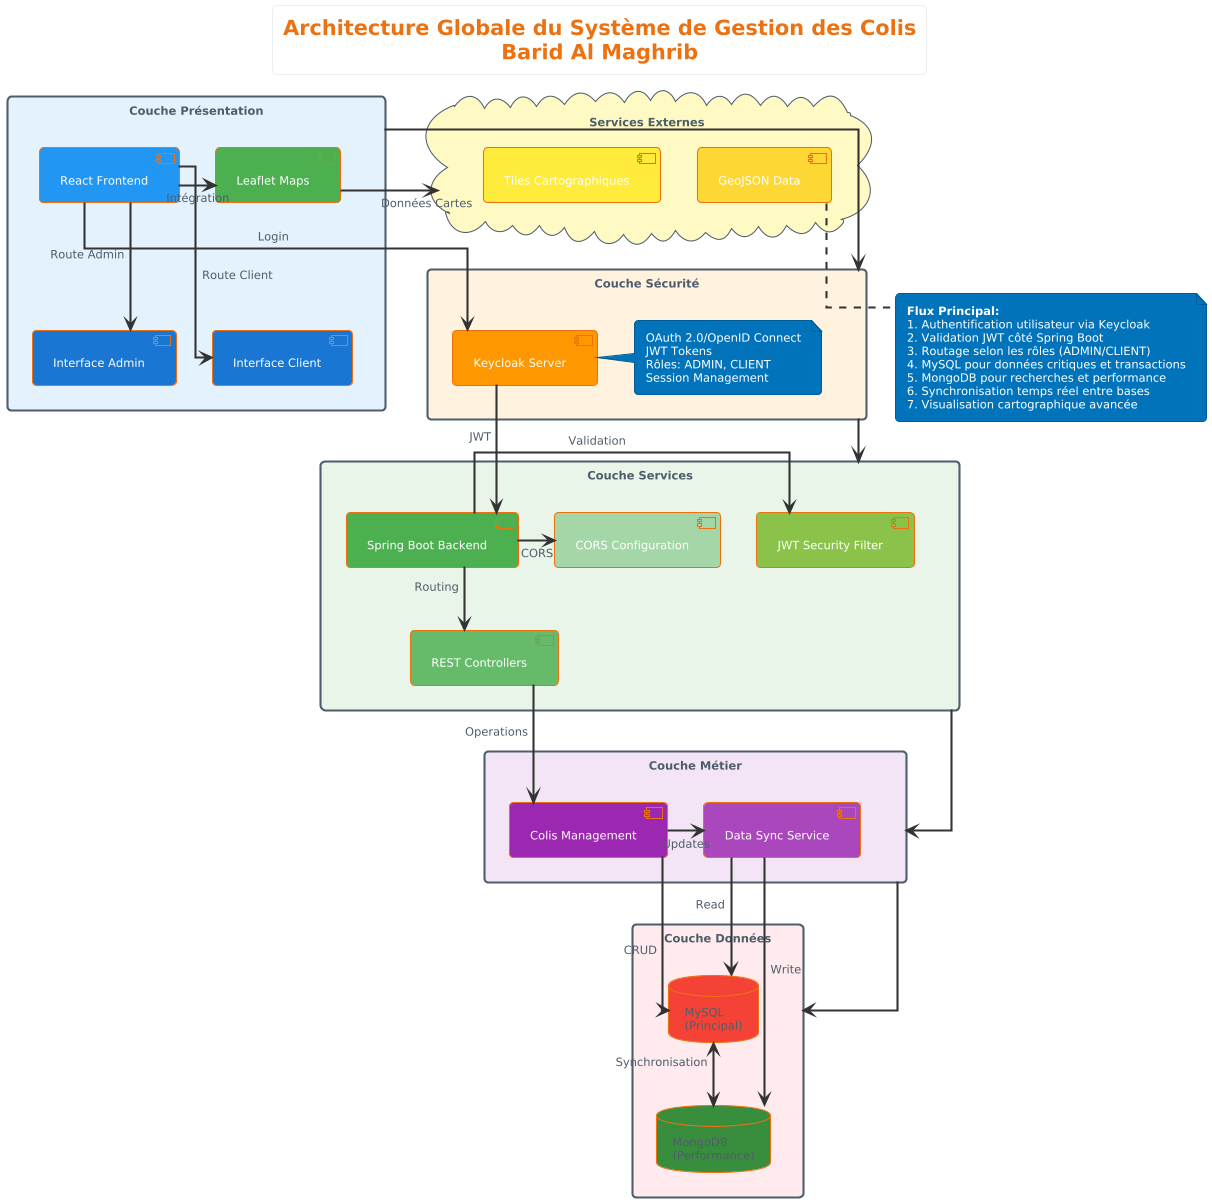
\includegraphics[width=0.8\textwidth]{images/architecture_globale.png}
\caption{Architecture globale du système hybride}
\label{fig:architecture_globale}
\end{figure}
La Figure \ref{fig:architecture_globale} présente l'architecture complète du système avec les flux de données et les interactions entre composants. La couche de présentation, développée en React, implémente une Single Page Application moderne avec gestion d'état centralisée et communication asynchrone avec les services backend via des API REST sécurisées.

La couche métier, architecturée autour de Spring Boot, expose des API REST [14] sécurisées par Keycloak et implémente la logique business complexe. Cette couche intègre le routage intelligent des requêtes vers les systèmes de persistance appropriés selon la nature des opérations : consultation rapide via MongoDB pour les listings et recherches, opérations transactionnelles via MySQL pour les modifications et la cohérence des données.

La couche de persistance hybride constitue l'innovation principale de cette architecture. MongoDB sert de cache intelligent et de moteur de recherche pour les opérations de consultation haute performance, tandis que MySQL conserve le rôle de source de vérité pour les données transactionnelles critiques. Un service de synchronisation automatique maintient la cohérence entre les deux systèmes en temps réel.

L'intégration de Keycloak [8] comme Identity and Access Management (IAM) centralise l'authentification et l'autorisation, supportant les standards OAuth 2.0 [11] et OpenID Connect [12]. Cette architecture sécurisée garantit l'isolation des données clients et la gestion fine des rôles utilisateur.

\subsection{Patterns architecturaux}

L'architecture s'appuie sur plusieurs patterns éprouvés adaptés aux spécificités du domaine postal. Le pattern Repository abstrait l'accès aux données en fournissant une interface unifiée indépendante du système de persistance sous-jacent. Cette approche facilite les tests unitaires et permet l'évolution future des choix technologiques.

Le pattern Strategy gouverne le routage des requêtes entre MySQL et MongoDB selon des critères définis : type d'opération, volume de données, exigences de cohérence. Cette stratégie s'adapte dynamiquement aux conditions d'utilisation et peut évoluer selon l'expérience opérationnelle.

Le pattern Observer est implémenté pour la synchronisation des données entre les systèmes de persistance. Les modifications effectuées sur MySQL déclenchent automatiquement la mise à jour des données correspondantes dans MongoDB, garantissant la cohérence sans impact sur les performances utilisateur.

Le pattern Facade simplifie l'interface des services complexes en exposant des API métier de haut niveau masquant la complexité technique de l'architecture hybride. Cette approche préserve la simplicité d'usage pour les développeurs frontend tout en exploitant la richesse technique du backend.

\subsection{Choix technologiques}

Les choix technologiques s'appuient sur des critères de maturité, performance, et écosystème pour garantir la pérennité de la solution. Spring Boot 3.0 constitue le framework backend principal, bénéficiant d'un écosystème riche et d'une communauté active. L'intégration native avec Spring Security facilite l'implémentation des exigences de sécurité enterprise.

MongoDB 6.0 est retenu pour la couche de cache et de recherche, exploitant ses capacités d'indexation full-text et de requêtage flexibles. Les fonctionnalités d'agrégation native permettent la génération efficace de statistiques sans impact sur les performances de consultation.

Keycloak s'impose comme solution d'authentification et d'autorisation, apportant les standards OAuth 2.0/OpenID Connect et une gestion centralisée des identités. Cette solution enterprise offre la scalabilité et les fonctionnalités avancées requises pour un opérateur de l'envergure de Barid Al Maghrib.

React 18 avec TypeScript structure le frontend moderne, exploitant les dernières innovations de performance (Concurrent Features, Suspense) et de développement productif. L'intégration de Leaflet et des librairies cartographiques spécialisées enrichit considérablement les capacités de visualisation géographique.

\section{Modélisation UML}

\subsection{Diagrammes de cas d'utilisation}

La modélisation des cas d'utilisation identifie deux acteurs principaux interagissant avec le système selon des profils d'usage distincts. L'acteur Client représente les expéditeurs utilisant les services de Barid Al Maghrib et nécessitant l'accès à leurs données d'expédition. L'acteur Administrateur dispose de privilèges étendus pour la supervision globale du système..

\begin{figure}[H]
\centering
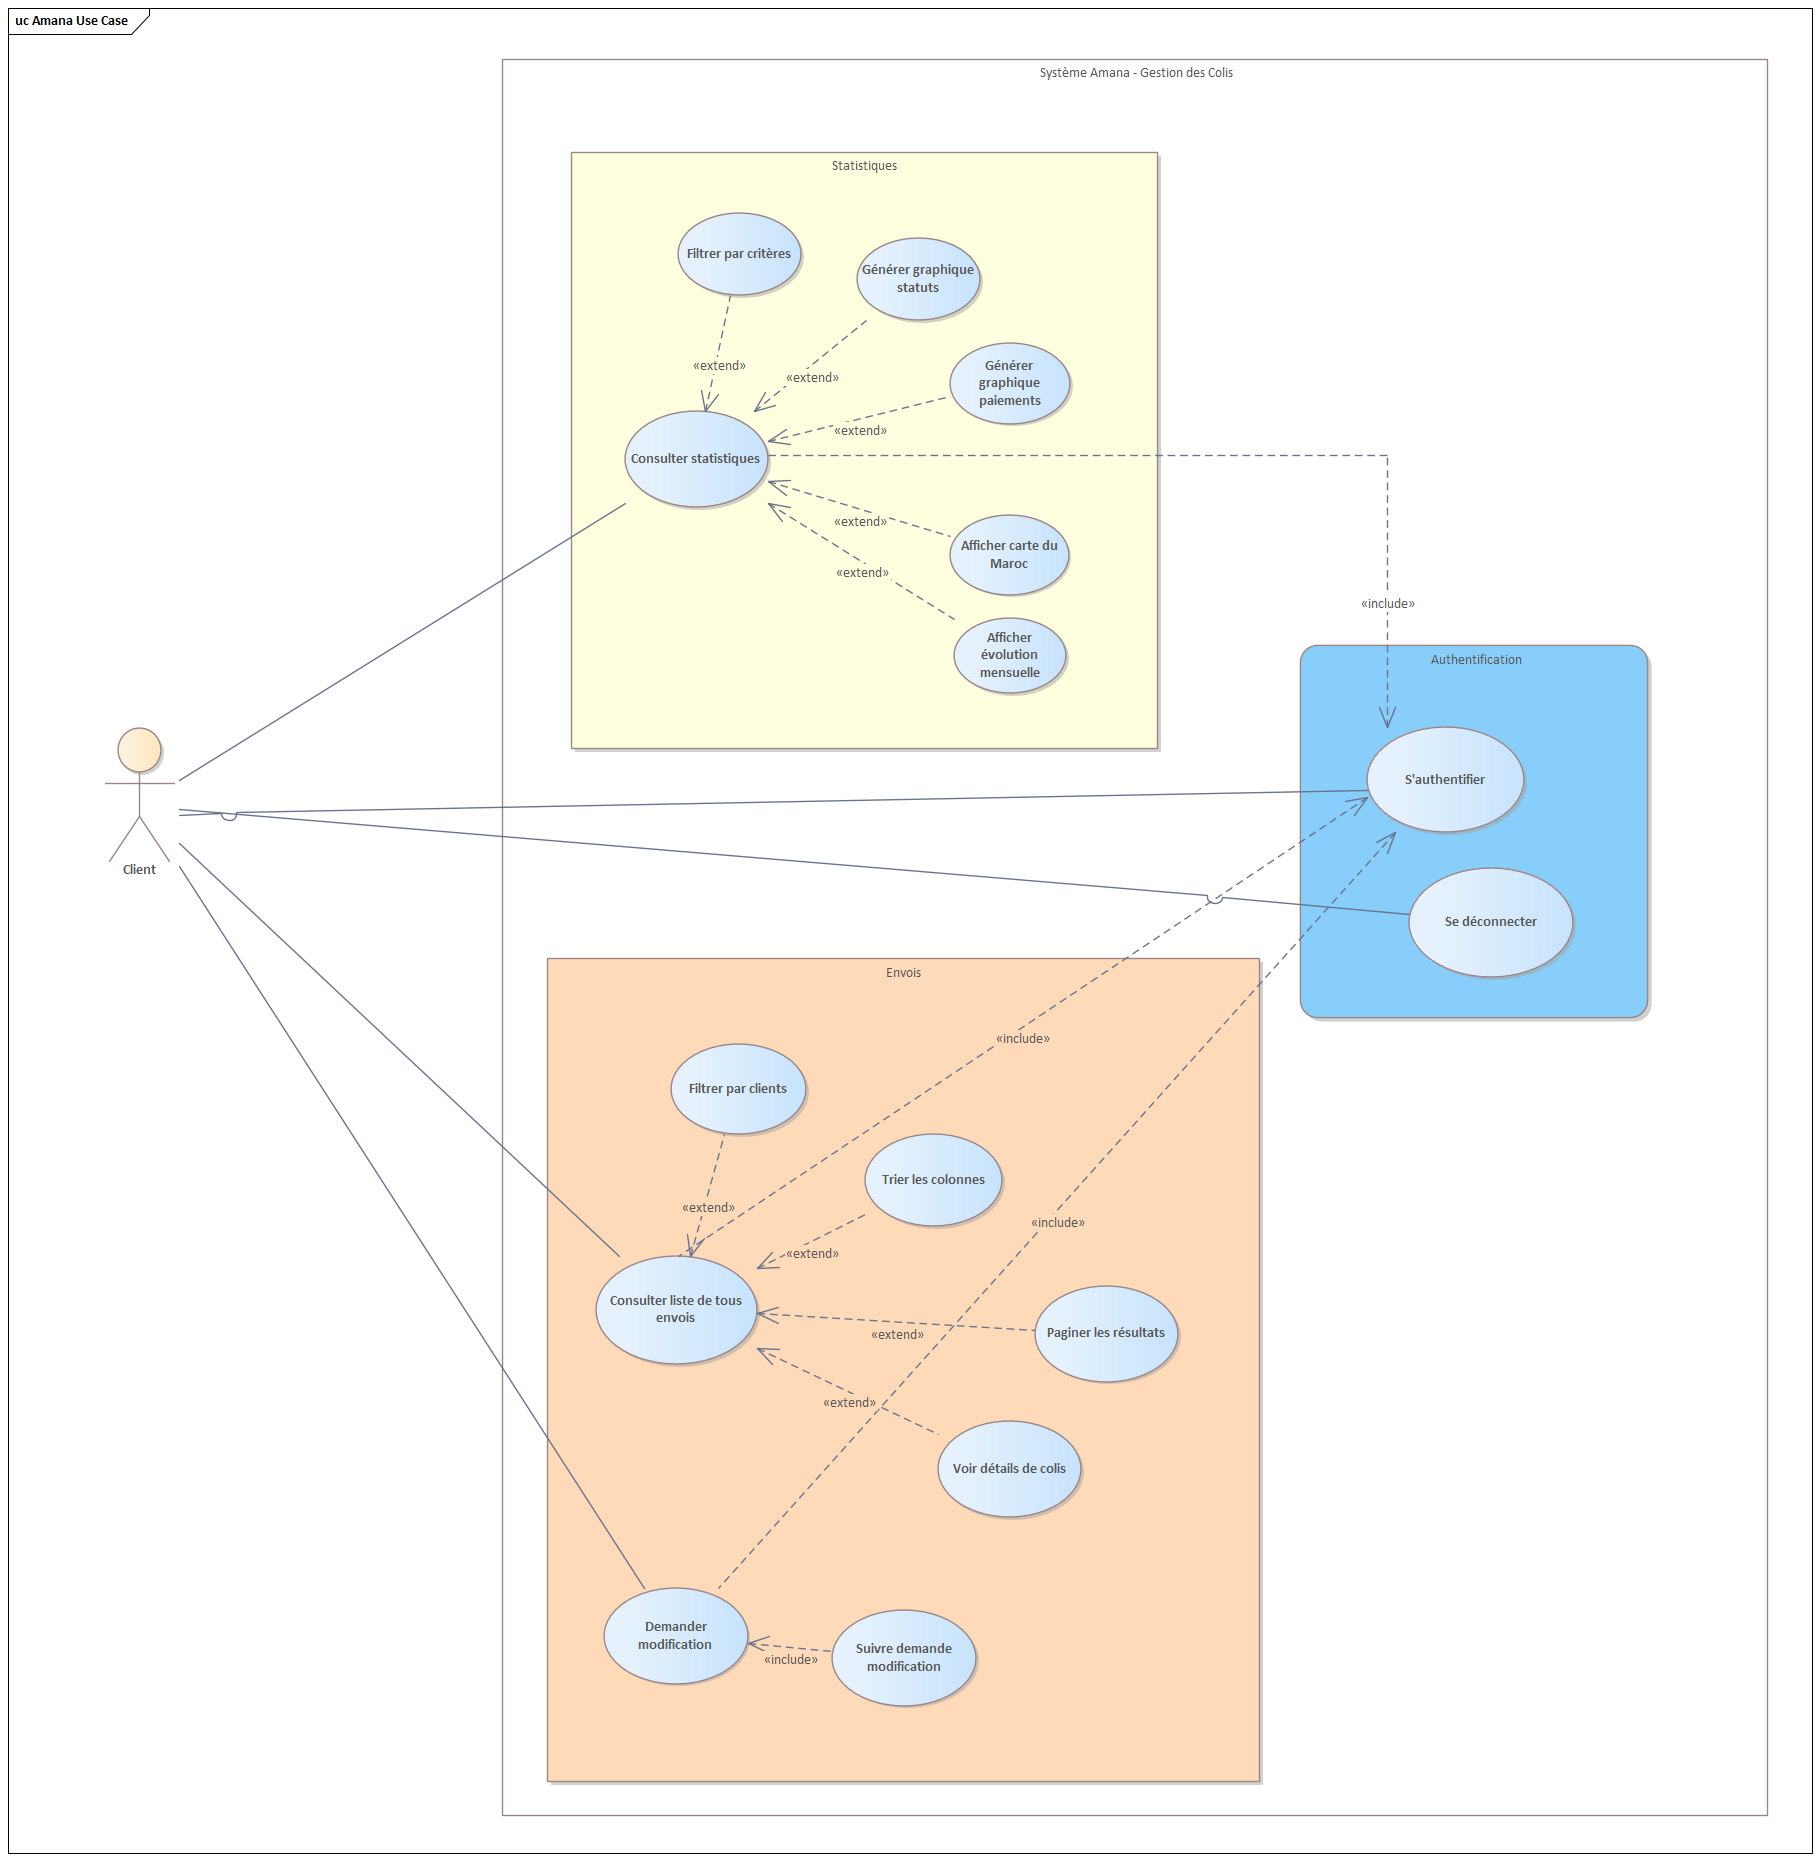
\includegraphics[width=0.8\textwidth]{images/Amana Colis Use Case Client.png}
\caption{Diagramme de cas d'utilisation - Acteur Client}
\label{fig:use_case_client}
\end{figure}

La Figure \ref{fig:use_case_client} présente les cas d'utilisation accessibles à l'acteur Client. Ce dernier peut consulter ses colis avec des capacités de filtrage et de recherche avancées, accéder aux détails individuels de chaque envoi, soumettre des demandes de modification pour les informations non critiques, et générer des statistiques personnalisées de son activité d'expédition.

\begin{figure}[H]
\centering
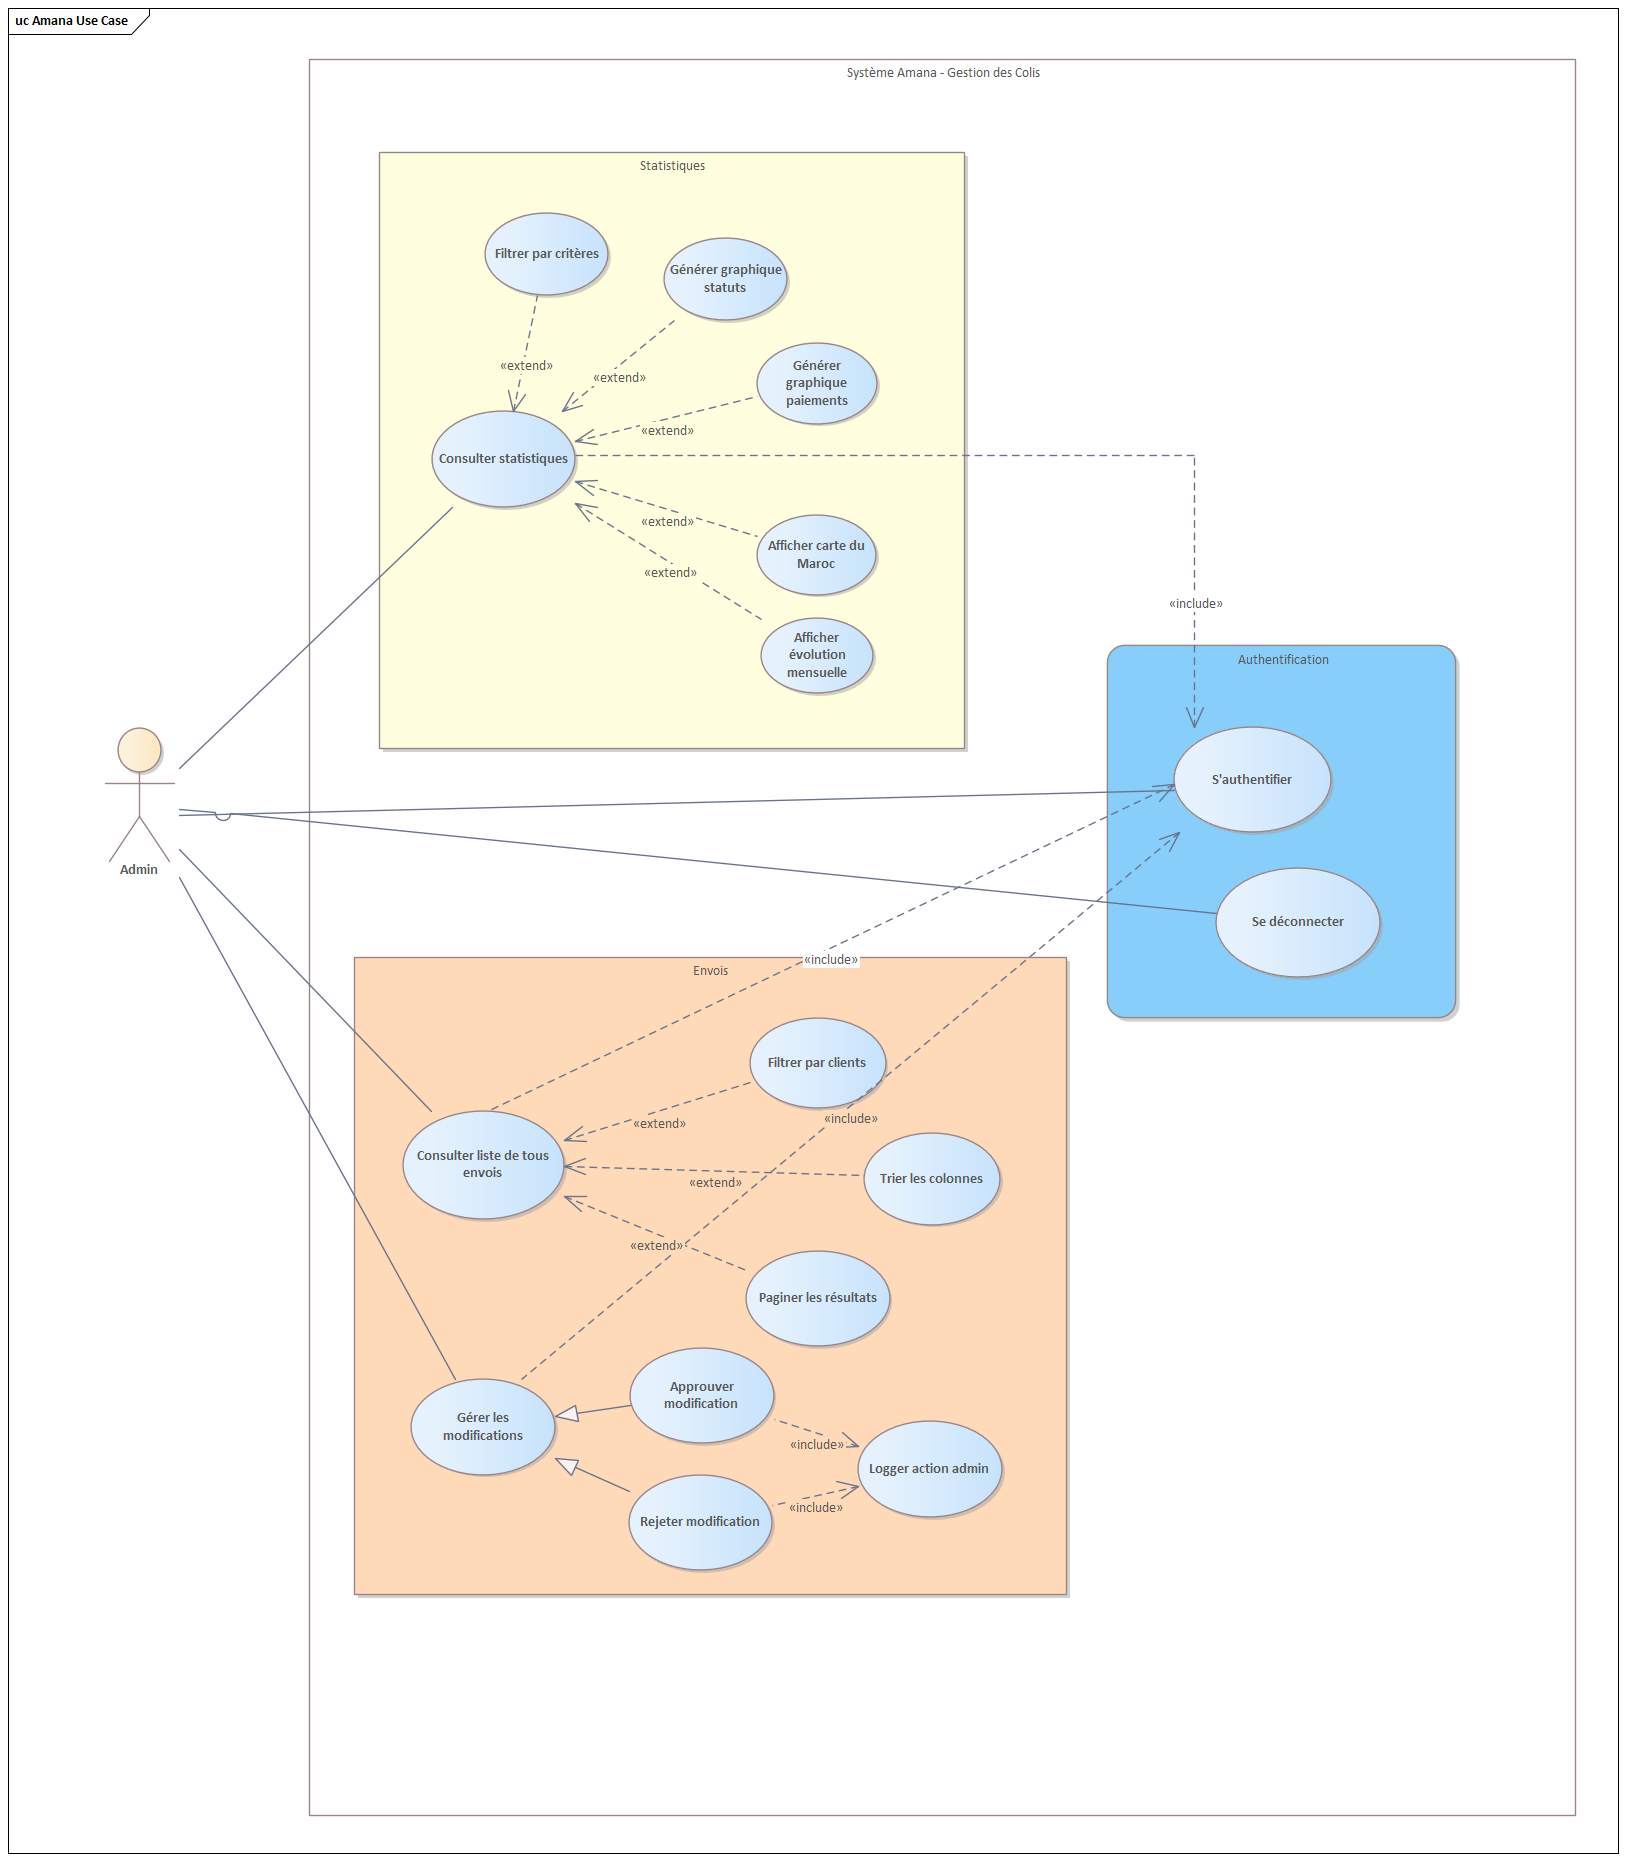
\includegraphics[width=0.8\textwidth]{images/Amana Colis Use Case Admin.png}
\caption{Diagramme de cas d'utilisation - Acteur Administrateur}
\label{fig:use_case_admin}
\end{figure}

La Figure \ref{fig:use_case_admin} détaille les privilèges étendus de l'acteur Administrateur. Il dispose d'un accès global à l'ensemble des données colis tous clients confondus, peut valider ou rejeter les demandes de modification avec traçabilité complète.

\subsection{Diagrammes de séquence}

Le diagramme de séquence de consultation des colis illustre l'orchestration complexe entre les différents composants du système hybride, mettant en évidence l'intégration de Keycloak pour l'authentification et le routage intelligent vers MongoDB pour l'optimisation des performances.

\begin{figure}[H]
\centering
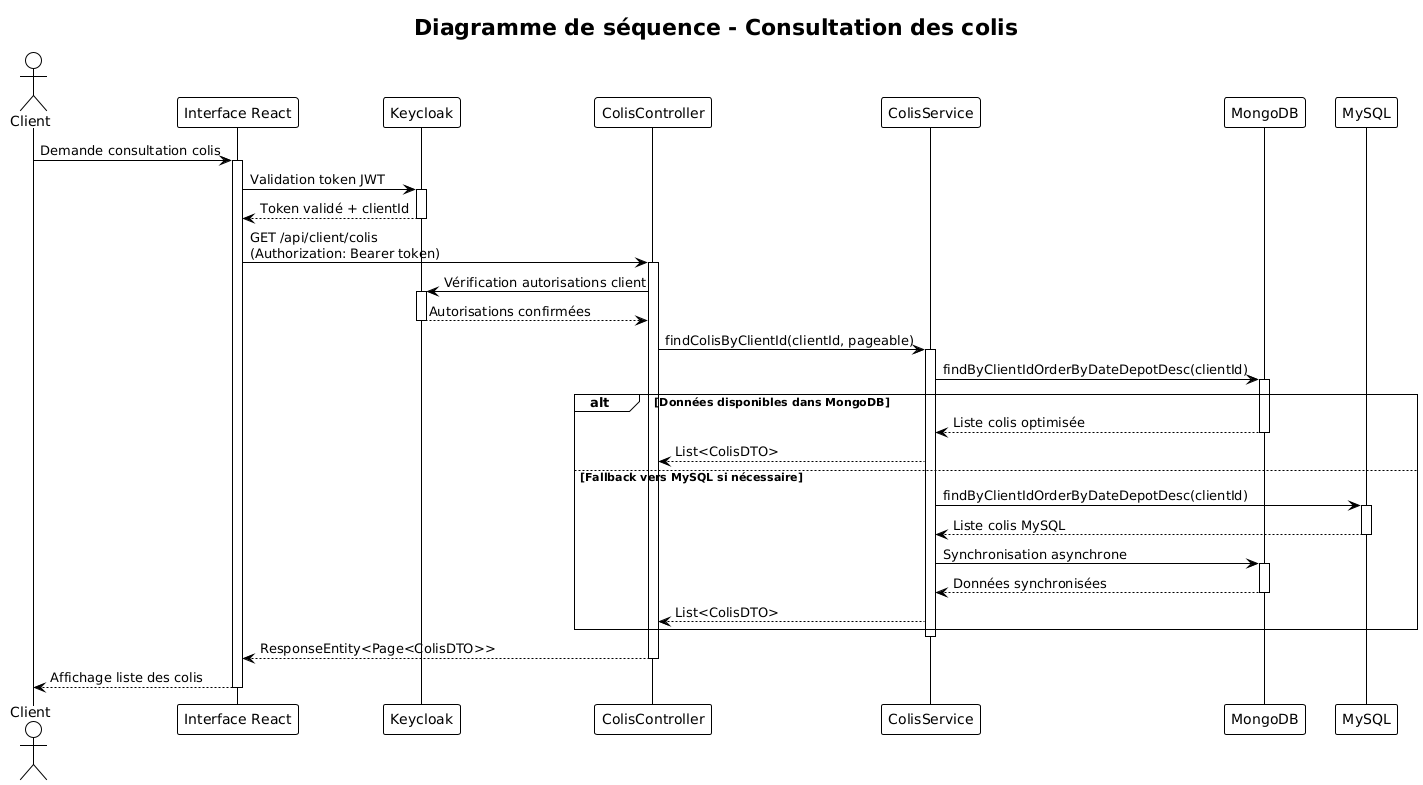
\includegraphics[width=1.0\textwidth]{images/sequence_consultation.png}
\caption{Diagramme de séquence - Consultation des colis}
\label{fig:sequence_consultation}
\end{figure}
La Figure \ref{fig:sequence_consultation} montre l'interaction complète depuis l'authentification utilisateur jusqu'à l'affichage des données. Le processus débute par la validation du token JWT via Keycloak, suivi de la vérification des autorisations client. La requête est ensuite routée vers MongoDB pour récupération optimisée des données de listing, avec fallback vers MySQL si nécessaire.

\begin{figure}[H]
\centering
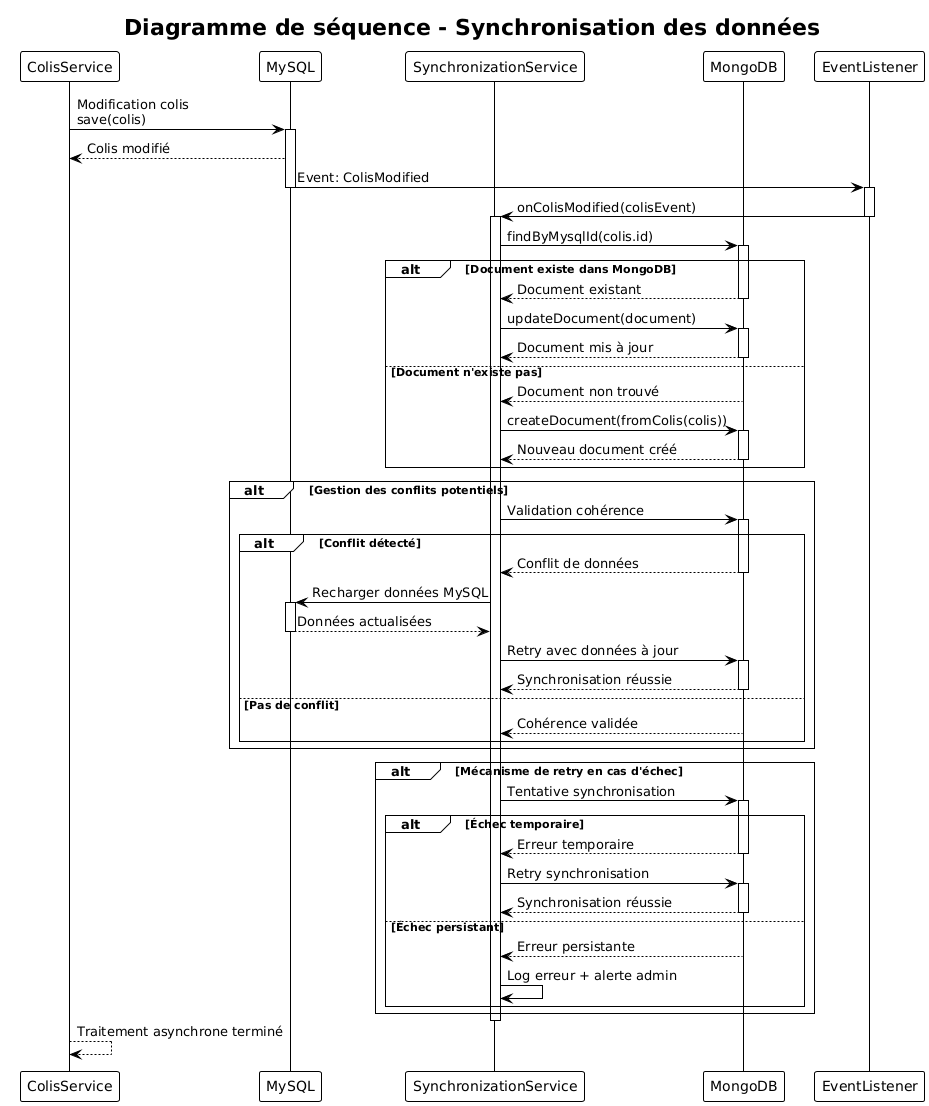
\includegraphics[width=0.9\textwidth]{images/sequence_synchronisation.png}
\caption{Diagramme de séquence - Synchronisation des données}
\label{fig:sequence_synchronisation}
\end{figure}
La Figure \ref{fig:sequence_synchronisation} modélise le processus critique de maintien de cohérence entre MySQL et MongoDB. Toute modification sur MySQL déclenche un événement traité asynchronement par le service de synchronisation, qui met à jour les documents correspondants dans MongoDB avec gestion des conflits potentiels et mécanismes de retry en cas d'échec.

\subsection{Diagrammes de classes}

La modélisation objet identifie les entités métier principales et leurs relations, ainsi que les classes techniques nécessaires à l'implémentation de l'architecture hybride.

\begin{figure}[H]
\centering
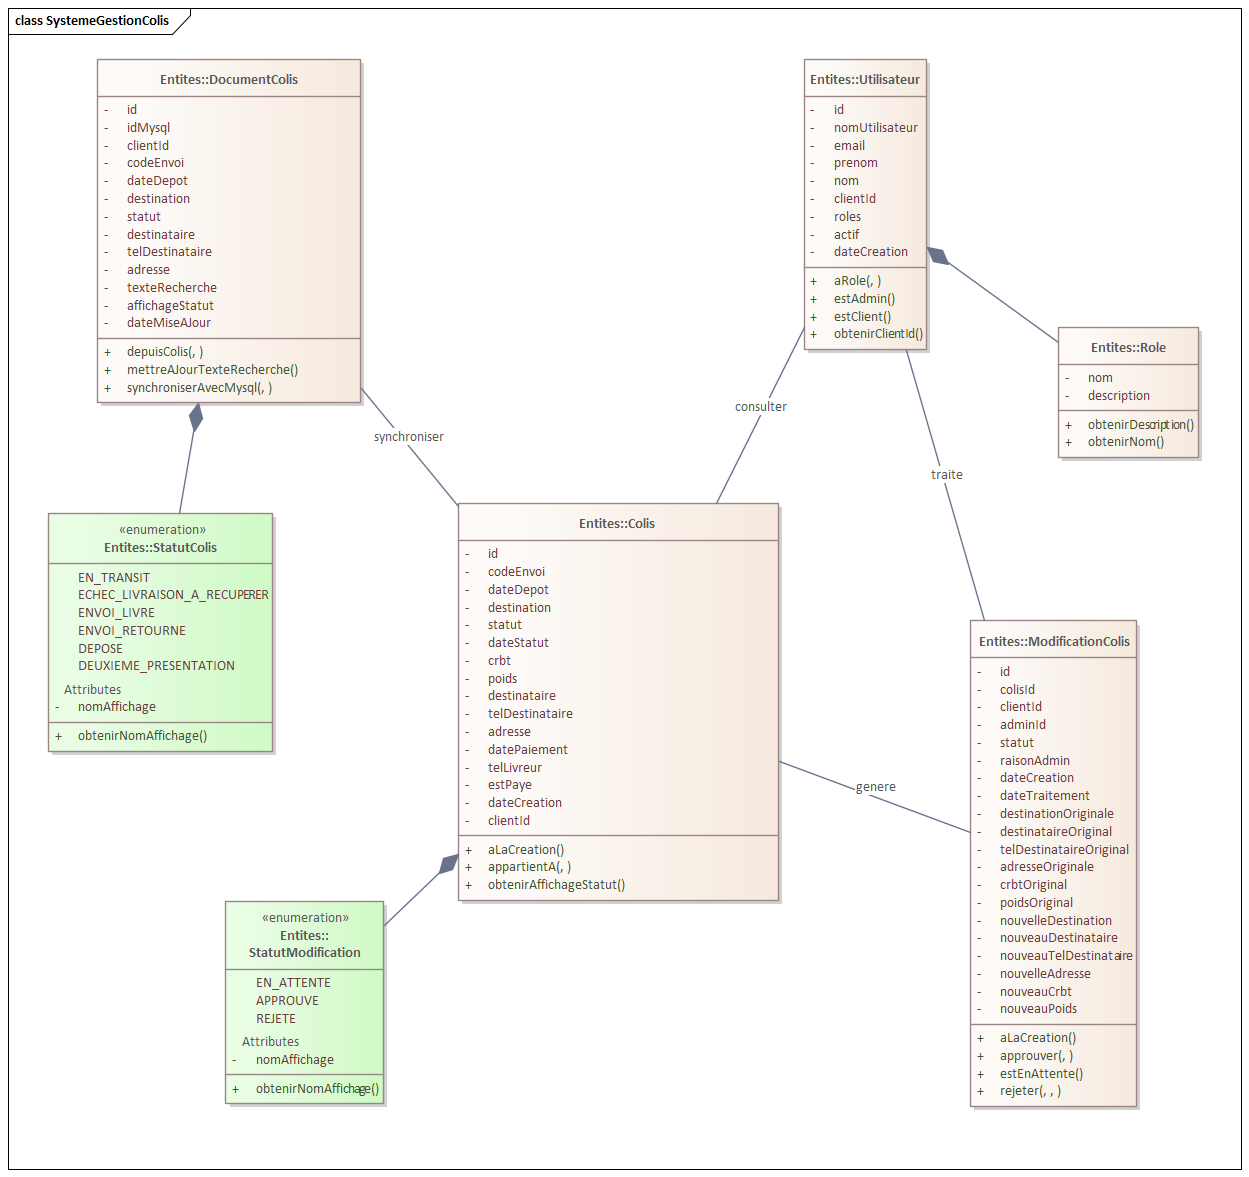
\includegraphics[width=1.1\textwidth]{images/class_diagram.png}
\caption{Diagramme de classes principal}
\label{fig:class_diagram}
\end{figure}

La Figure \ref{fig:class_diagram} présente la structure objet du système avec les entités métier centrales. La classe \texttt{Colis} constitue l'entité principale encapsulant l'ensemble des informations descriptives. La classe \texttt{Utilisateur} modélise les expéditeurs avec ses attributions d'identification et autorisations d'accès. La classe \texttt{ColisModification} gère le workflow d'approbation des demandes de changement.
\newpage
\subsection{Modèle de données}

Le modèle de données hybride concilie les paradigmes relationnels et documentaires pour optimiser les différents patterns d'accès selon les besoins fonctionnels identifiés.

\begin{figure}[H]
\centering
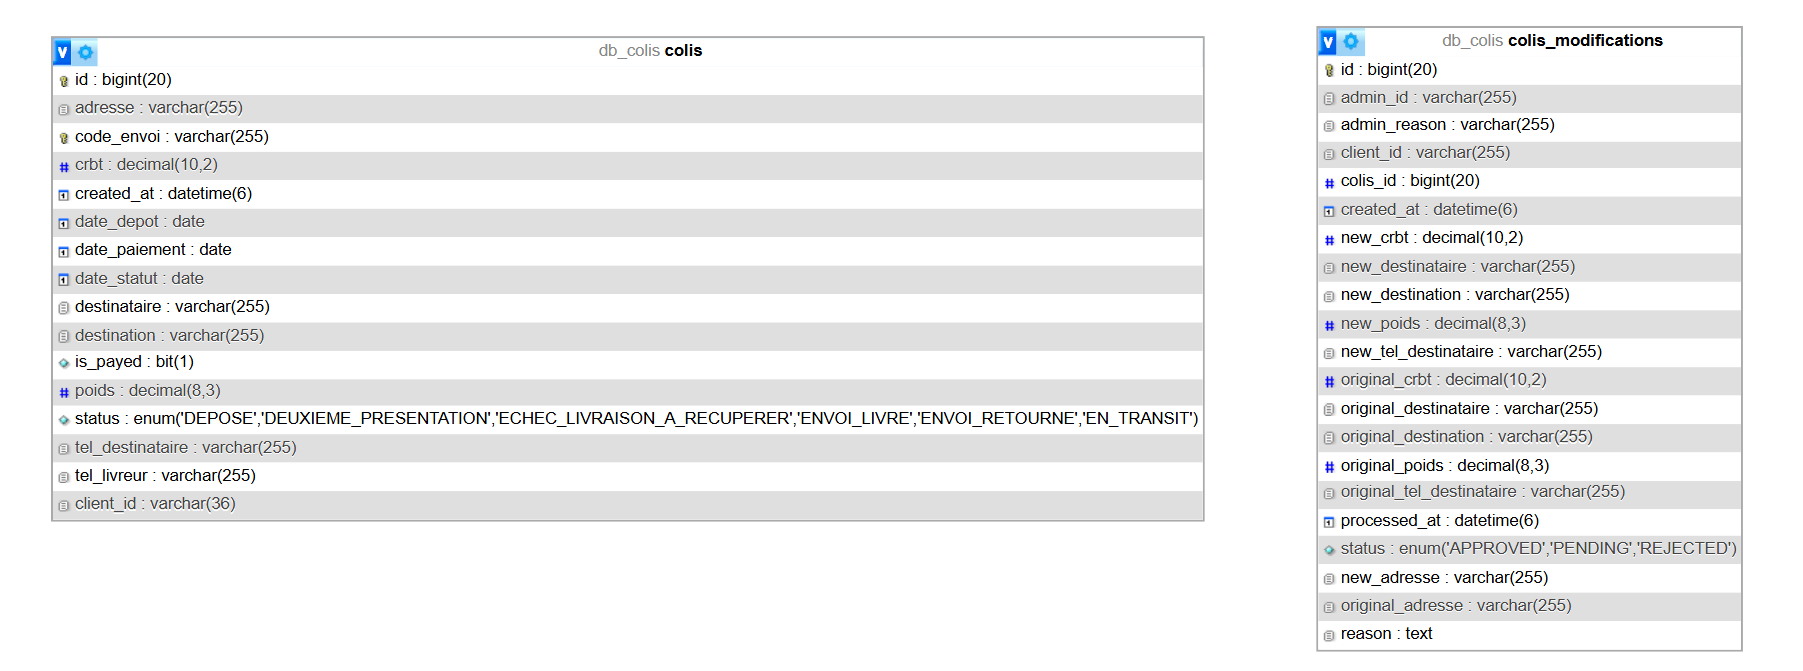
\includegraphics[width=1.0\textwidth]{images/data_model_mysql.png}
\caption{Modèle de données MySQL}
\label{fig:data_model_mysql}
\end{figure}
La Figure \ref{fig:data_model_mysql} illustre la structure relationnelle MySQL avec les tables principales et leurs relations. Le modèle normalisé garantit l'intégrité transactionnelle avec les contraintes d'intégrité référentielle appropriées. Les index composites optimisent les requêtes fréquentes tout en préservant les performances des opérations transactionnelles.

\section{Conception de la Base de Données}

\subsection{Modèle relationnel (MySQL)}

Le modèle relationnel MySQL préserve la structure normalisée garantissant l'intégrité transactionnelle et la cohérence des données critiques pour les opérations de Barid Al Maghrib.

\begin{figure}[H]
\centering
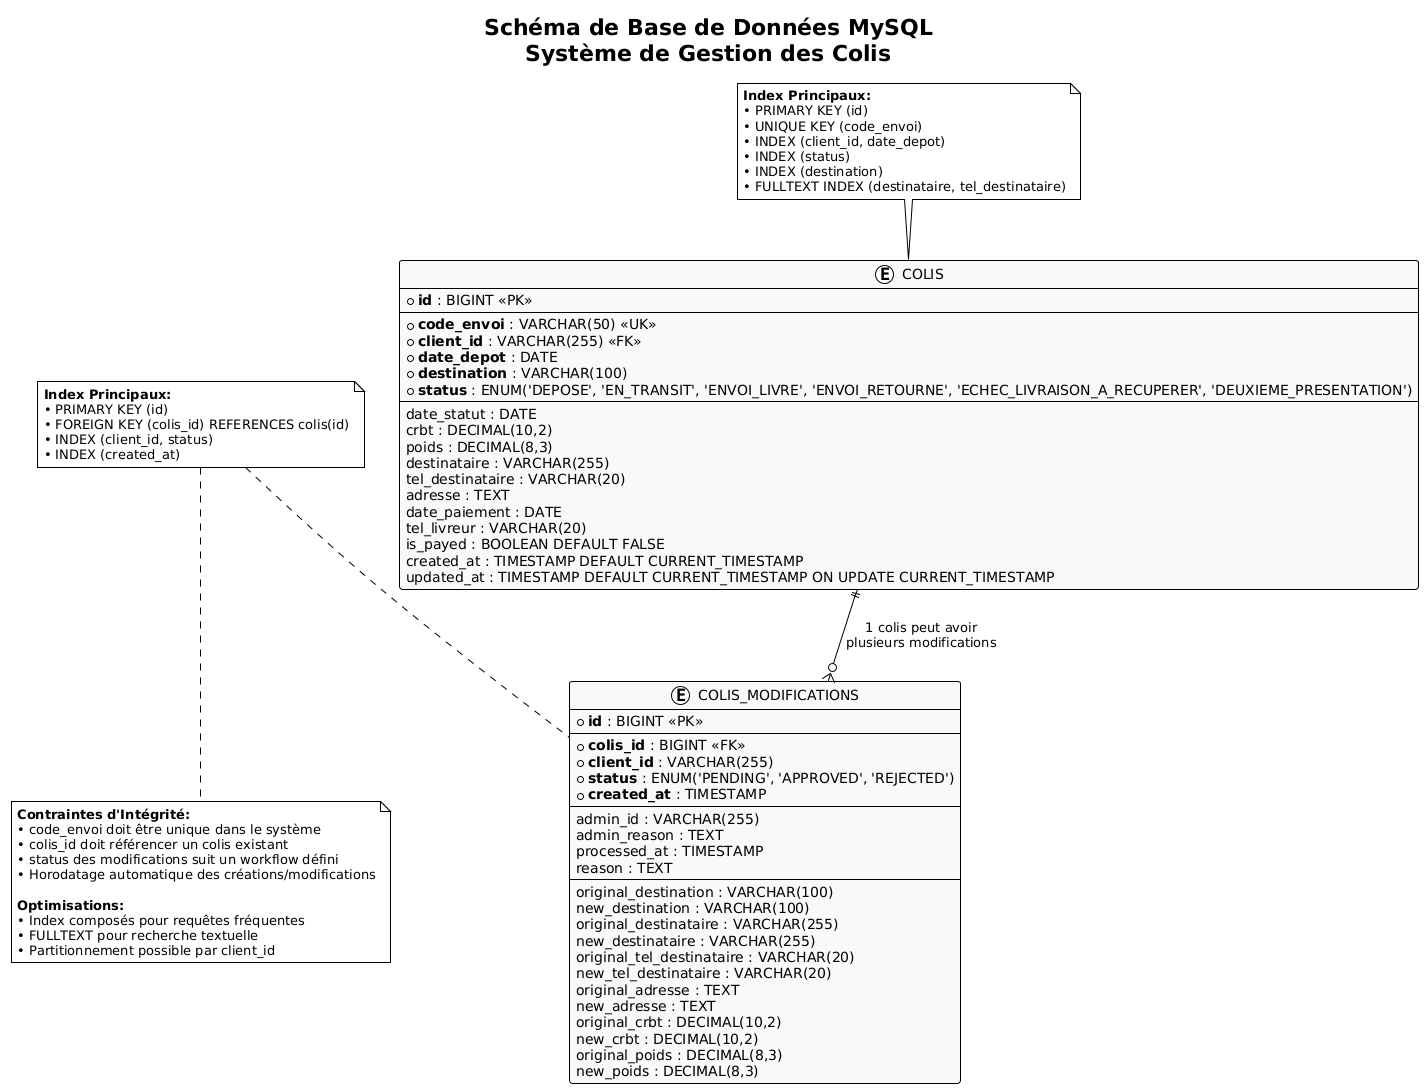
\includegraphics[width=1.0\textwidth]{images/mysql_schema.png}
\caption{Schéma de base de données MySQL}
\label{fig:mysql_schema}
\end{figure}

La Figure \ref{fig:mysql_schema} présente la structure détaillée de la base MySQL avec les contraintes d'intégrité référentielle. La table \texttt{colis} constitue l'entité principale avec ses attributs obligatoires : \texttt{id}, \texttt{code\_envoi}, \texttt{client\_id}, \texttt{date\_depot}, \texttt{destination}, \texttt{status}. La table \texttt{colis\_modifications} modélise le workflow d'approbation des changements avec conservation de l'historique complet.

L'optimisation des performances MySQL s'appuie sur une stratégie d'indexation ciblée : index composites sur \texttt{(client\_id, date\_depot)} pour les consultations client, index sur \texttt{status} et \texttt{destination} pour les filtres administrateur, index full-text sur les champs de recherche textuelle.

\subsection{Modèle NoSQL (MongoDB)}

Le modèle documentaire MongoDB privilégie la dénormalisation pour optimiser les performances de lecture et simplifier les requêtes de consultation utilisateur quotidiennes.

\begin{figure}[H]
\centering
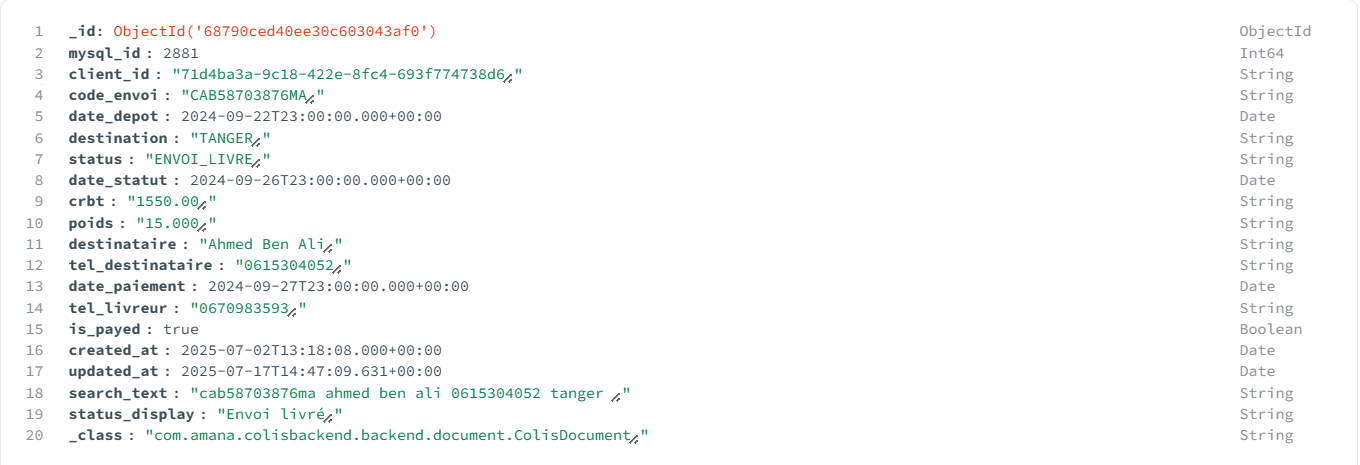
\includegraphics[width=1.3\textwidth]{images/mongodb_document.png}
\caption{Structure des documents MongoDB}
\label{fig:mongodb_document}
\end{figure}

La Figure \ref{fig:mongodb_document} illustre la structure documentaire optimisée avec les champs calculés et les index spécialisés. Les documents intègrent l'ensemble des informations nécessaires aux vues listing, éliminant les jointures coûteuses. La stratégie d'indexation exploite les spécificités NoSQL : index composés sur \texttt{(clientId, dateDepot)}, index text sur \texttt{search\_text}, index géospatiaux pour les requêtes cartographiques.
